% source TikZ and PGF manual
% modified by Truong Nhan Nguyen

\documentclass[tikz, border=10pt]{standalone}

% preamble
\usepackage{tikz}
\usetikzlibrary{arrows, snakes, backgrounds, petri}
\usepackage{amsmath, amsfonts, amssymb, mathtools}
\usepackage{mathpazo}

% define styles
\tikzset{
    % node styles
    place/.style = {minimum size=6mm, thick, draw=blue!75, fill=blue!20, circle},
    transition/.style = {minimum size=4mm, thick, draw=black!75, fill=black!20},
    red place/.style = {place, draw=red!75, fill=red!20},
    % arrow style
    pre/.style={<-, shorten <=1pt, semithick, >=stealth'},
    post/.style={->, shorten >=1pt, semithick, >=stealth'},
    % label style
    every label/.style={red}
}

\begin{document}
    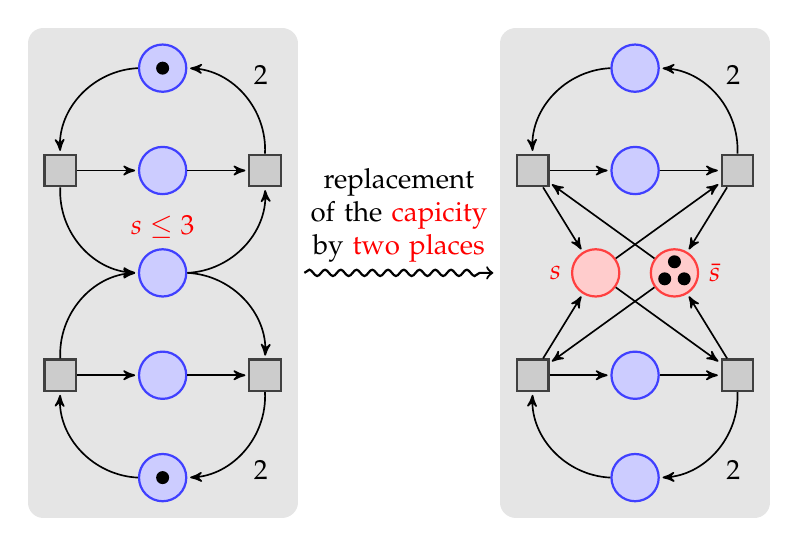
\begin{tikzpicture}[node distance=1.3 cm, auto, bend angle=45]
        % first net
        \node[place, tokens=1] (w1) {};
        \node[place] (c1) [below of=w1] {};
        \node[place] (s) [below of=c1, label=above:$s \le 3$] {};
        \node[place] (c2) [below of=s] {};
        \node[place, tokens=1] (w2) [below of=c2] {};
        
        \node[transition] (e1) [left of=c1] {}
            edge[pre, bend left] (w1)
            edge[post] (c1)
            edge[post, bend right] (s);
            
        \node[transition] (e2) [left of=c2] {}
            edge[post, bend left] (s)
            edge[post] (c2)
            edge[pre, bend right] (w2);
            
        \node[transition] (l1) [right of=c1] {}
            edge[post, bend right] node[swap] {$2$} (w1)
            edge[pre] (c1)
            edge[pre, bend left] (s);
            
        \node[transition] (l2) [right of=c2] {}
            edge[pre, bend right] (s)
            edge[pre] (c2)
            edge[post, bend left] node {$2$} (w2);
        
        % second net
        \begin{scope}[xshift=6cm]
            \node[place] (w1') {};
            \node[place] (c1') [below of=w1'] {};
            \node[red place] (s1') [below of=c1', xshift=-5mm, label=left:$s$] {};
            \node[red place, tokens=3] (s2') [below of=c1', xshift=5mm, label=right:$\bar s$]{};
            \node[place] (c2') [below of=s2', xshift=-5mm] {};
            \node[place] (w2') [below of=c2'] {};
            
            \node[transition] (e1') [left of=c1'] {}
                edge[pre, bend left] (w1')
                edge[post] (c1')
                edge[pre] (s2')
                edge[post] (s1');
                
            \node[transition] (e2') [left of=c2'] {}
                edge[post] (s1')
                edge[pre] (s2')
                edge[post] (c2')
                edge[pre, bend right] (w2');
                
            \node[transition] (l1') [right of=c1'] {}
                edge[post, bend right] node[swap] {$2$} (w1')
                edge[pre] (c1')
                edge[pre] (s1')
                edge[post] (s2');
                
            \node[transition] (l2') [right of=c2'] {}
                edge[post] (s2')
                edge[pre] (s1')
                edge[pre] (c2')
                edge[post, bend left] node {$2$} (w2');
        \end{scope}
        
        % draw snake line and text
        \draw[-to, thick, snake=snake, segment amplitude=0.4mm, segment length=2mm, line after snake=1mm]
        ([xshift=5mm]s -| l1) -- ([xshift=-5mm]s1' -| e1')
        node[above, midway, text width=3cm, text centered]
        {replacement of the \textcolor{red}{capicity} by \textcolor{red}{two places}};
        
        % draw rectangle layers
        \begin{pgfonlayer}{background}
            \filldraw[line width=4mm, join=round, black!10]
             (w1.north -| l1.east) rectangle (w2.south -| e2.west)
             (w1'.north -| l1'.east) rectangle (w2'.south -| e2'.west);
        \end{pgfonlayer}
        
    \end{tikzpicture}
\end{document}